\def\QRCODE{TB_image_TUT.IMG.image_restoration_denoising_pythonqrcode.png}
\def\QRPAGE{http://www.iptutorials.science/tree/master/TB_image/TUT.IMG.image_restoration_denoising/python}
\pcorrectionsection{Python correction}

\begin{python}
import matplotlib.pyplot as plt
import numpy as np
from scipy import ndimage
from scipy import misc
\end{python}


\subsection{Generation of random noises}
In order to convert stretch the images into the range [0;1], the following function can be used:

\begin{python}
def hist_stretch(I):
    # histogram stretching
    # returns values of I linearly stretched to range [0;1]
    I = I - np.min(I);
    I = I / np.max(I);
    return I;
\end{python}


Random noise illustrations are proposed in Figs.\ref{fig:image_restoration_denoising:python:noises} and \ref{fig:image_restoration_denoising:python:histograms}, and a size $S=32$ is used to generate the noisy images.
\begin{figure}[ht]
 \centering\caption{Resulting noise images.}%
 \subfloat[Uniform noise.]{
\includegraphics[width=.42\linewidth]{uniform_noise.png}}
 \hfill
 \subfloat[Gaussian noise.]{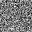
\includegraphics[width=.42\linewidth]{gaussian_noise.png}}
 
  \subfloat[Salt and pepper noise.]{
\includegraphics[width=.42\linewidth]{sp_noise.png}} \hfill
 \subfloat[Exponential noise.]{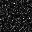
\includegraphics[width=.42\linewidth]{exponential_noise.png}}
\vspace*{-8pt}%
 \label{fig:image_restoration_denoising:python:noises}%
\end{figure}

\subsubsection{Uniform noise}
The python \minline{rand} function generates values between 0 and 1 with uniform distribution.

\begin{python}
S=32
a=0; b=255;
R1 = a + (b-a) * np.random.rand(S, S);
\end{python}

\subsubsection{Gaussian noise}
The python \minline{randn} function generates values with normal centered distribution.
\begin{python}
a=0; b=1;
R2 = a + (b-a)*np.random.randn(S, S);
\end{python}

\subsubsection{Salt and pepper noise}
\begin{python} 
a = 0.05; b = 0.1;
R3 = 0.5 * np.ones((S,S));
X = np.random.rand(S,S);
R3[X<=a] = 0;
R3[(X>a) & (X <= b)] = 1;
R3 = hist_stretch(R3);
\end{python}


\subsubsection{Exponential noise}
\begin{python}
a=1;
R4 = -1/a * np.log(1-np.random.rand(32, 32));
R4 = hist_stretch(R4); 
\end{python}

\begin{figure}[ht]
 \centering\caption{Histograms of the noise images generated with $32\times 32$ pixels.}%
 \subfloat[Uniform noise.]{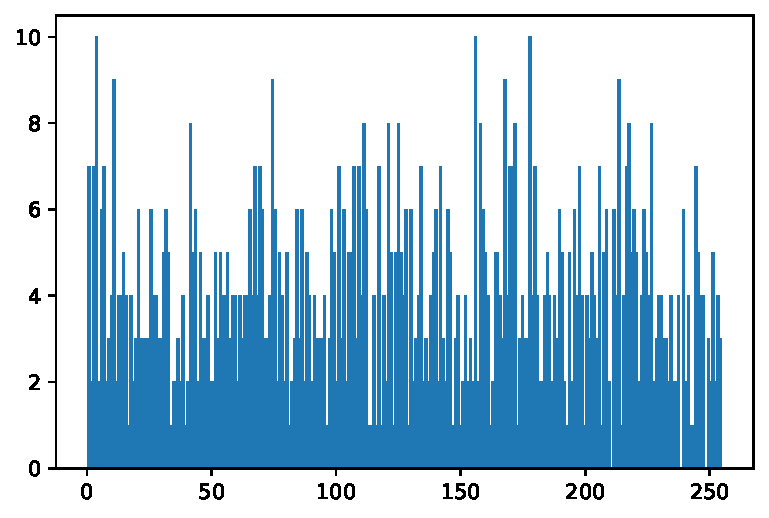
\includegraphics[width=.45\linewidth]{histo_uniform.pdf}}\hfill
 \subfloat[Gaussian noise.]{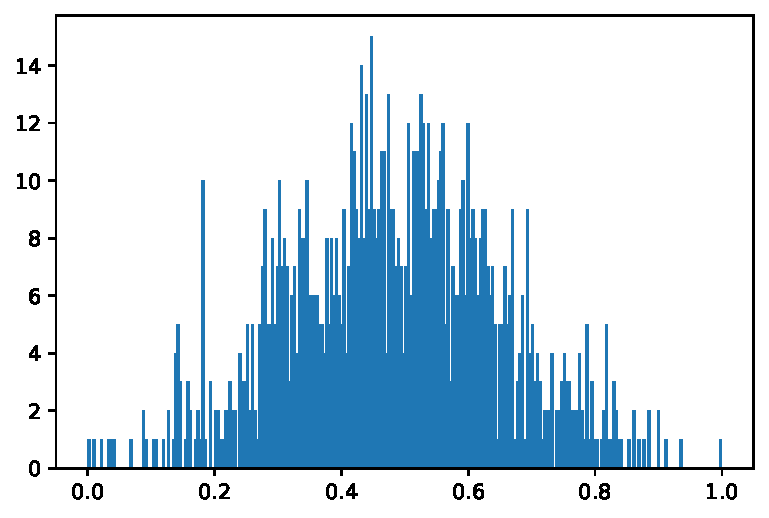
\includegraphics[width=.45\linewidth]{histo_gaussian.pdf}}
 
 \subfloat[Exponential noise.]{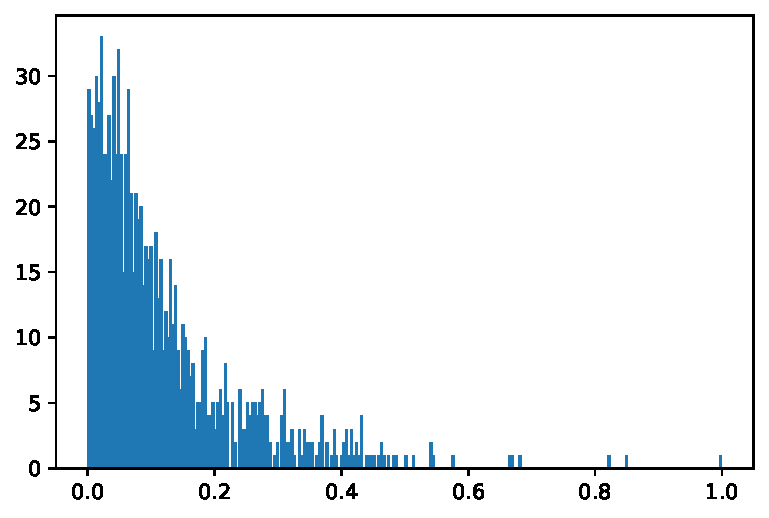
\includegraphics[width=.45\linewidth]{histo_exponential.pdf}}\hfill
 \subfloat[Salt and pepper noise.]{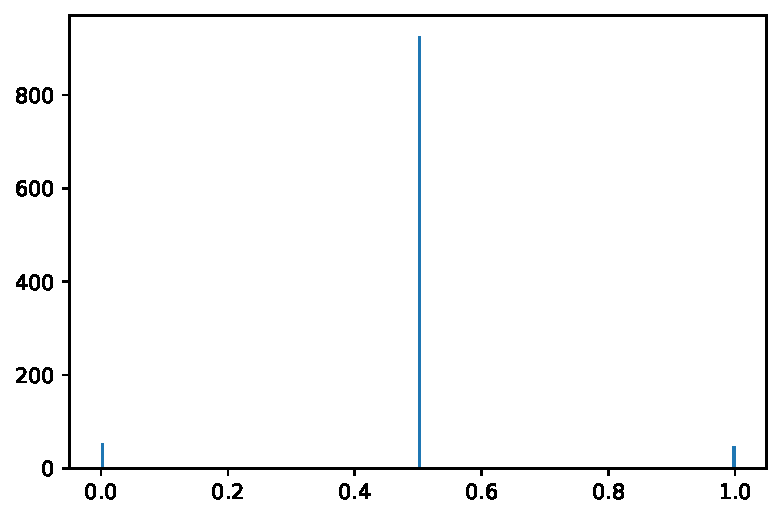
\includegraphics[width=.45\linewidth]{histo_sp.pdf}}%
 \label{fig:image_restoration_denoising:python:histograms}%
\end{figure}


\subsection{Noise estimation}
In order to estimate the noise, a ROI of visually constant gray level is chosen, and its histogram is displayed. This is simulated by the following code, the result is displayed in Fig.\ref{fig:image_restoration_denoising:python:histogram_roi}:

\begin{python}
# noise estimation
fig = plt.figure()
A = imageio.imread('jambe.png');
roi = A[160:200, 200:240];
plt.hist(roi.flatten(),255);
fig.savefig("histo_roi_leg.pdf", bbox_inches='tight');
\end{python}

Then, some noise is added to the image, and the histogram of the ROI is displayed. The results are observed in Figs.\ref{fig:image_restoration_denoising:python:hist_exp} and \ref{fig:image_restoration_denoising:python:hist_gauss}.
\begin{python}
# add exponential noise to image
nx, ny = A.shape;
expnoise = -1/.5 * np.log(1-np.random.rand(nx, ny));
expnoise = expnoise / np.max(expnoise);
B = A + 255*expnoise;
B = hist_stretch(B);
fig = plt.figure()
plt.imshow(B, cmap='gray');
imageio.imwrite("leg_exponential.png", B);
#plt.show()
\end{python}

\begin{python}
# add gaussian noise to image
nx, ny = A.shape;
gaussnoise = 50*np.random.rand(nx, ny);
B = A + gaussnoise;
B = hist_stretch(B);
fig = plt.figure()
plt.imshow(B, cmap='gray');
imageio.imwrite("leg_gaussian.png", B);
\end{python}

\begin{figure}[H]
\centering\caption{Histogram of the Region of Interest.}%
\subfloat[ROI.]{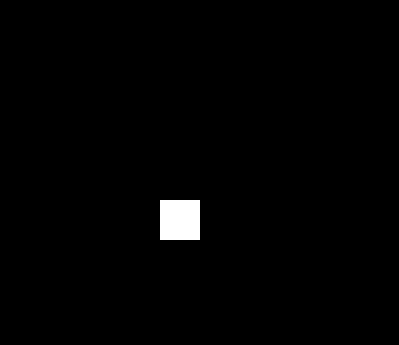
\includegraphics[width=.4\linewidth]{roi.png}} \hfill
\subfloat[Histogram.]{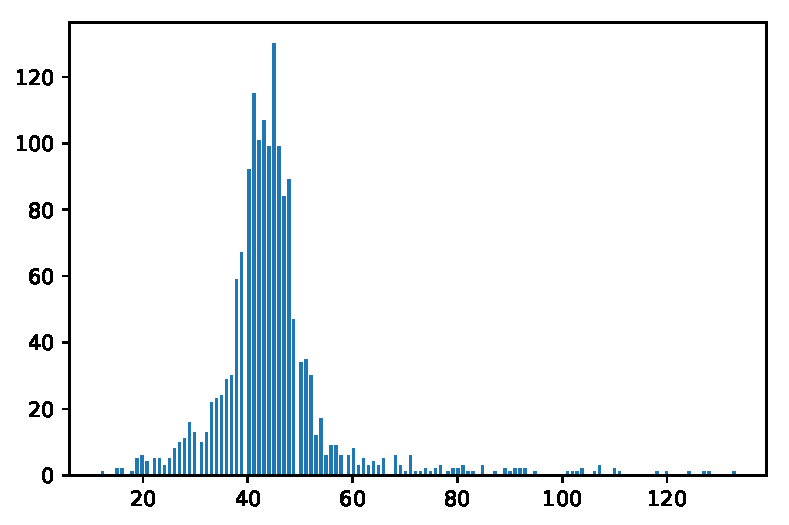
\includegraphics[width=.45\linewidth]{histo_roi_leg.pdf}}
\vspace*{-8pt}%
 \label{fig:image_restoration_denoising:python:histogram_roi}%
\end{figure}

\vspace*{-7pt}

In the case of exponential and Gaussian noise added to the image, The histograms are displayed in Figs.\ref{fig:image_restoration_denoising:python:hist_exp} and \ref{fig:image_restoration_denoising:python:hist_gauss}.

\vspace*{-7pt}

\begin{figure}[H]
 \centering\caption{Exponential noise.}%
 \subfloat[Addition of exponential noise to the original image of the leg.]{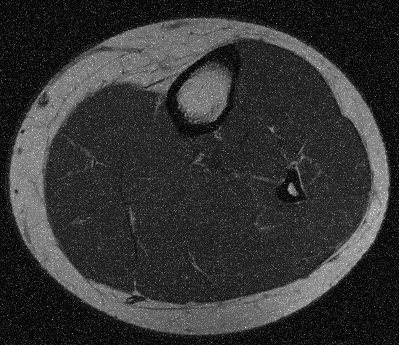
\includegraphics[width=.4\linewidth]{leg_exponential.png}}\hfill
  \subfloat[Histogram of the ROI.]{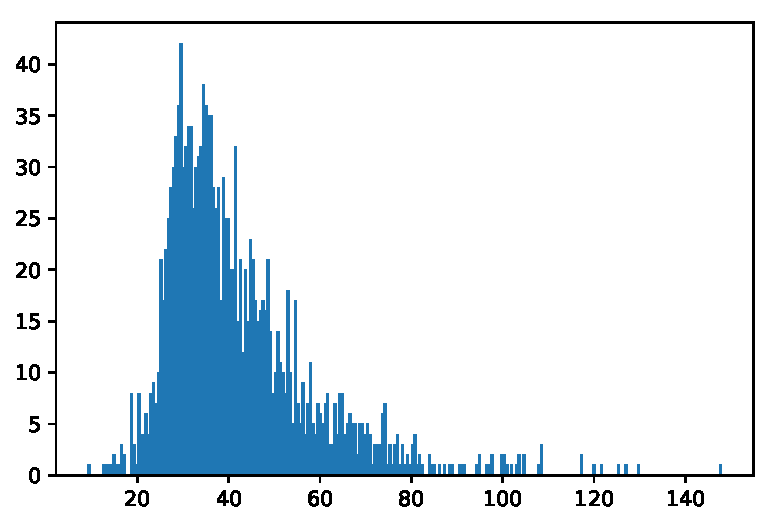
\includegraphics[width=.45\linewidth]{hist_exp.pdf}}%
\vspace*{-8pt}%
  \label{fig:image_restoration_denoising:python:hist_exp}%
\end{figure}

\vspace*{-15pt}

\begin{figure}[H]
 \centering\caption{Gaussian noise.}%
 \subfloat[Addition of Gaussian noise to the original image of the leg.]{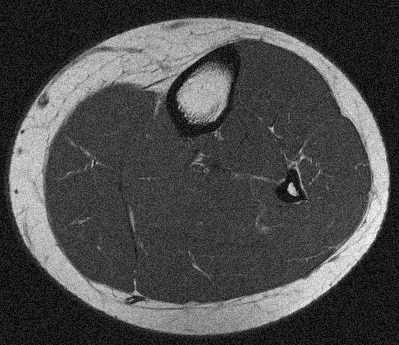
\includegraphics[width=.4\linewidth]{leg_gaussian.png}}\hfill
  \subfloat[Histogram of the ROI.]{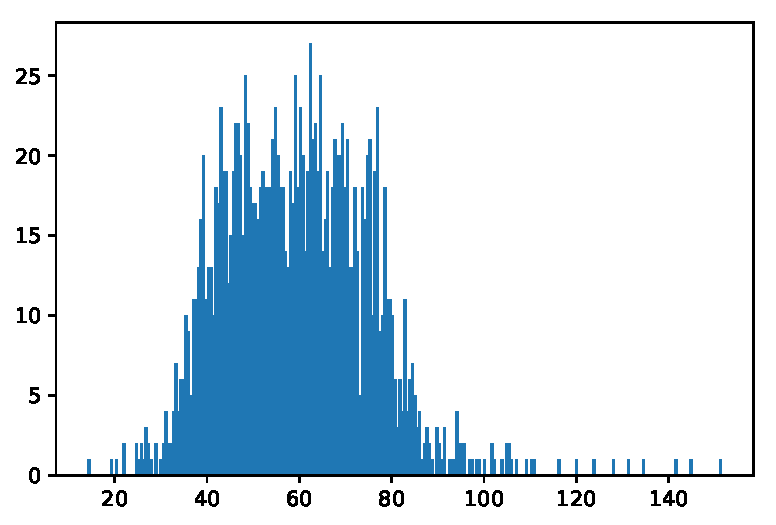
\includegraphics[width=.45\linewidth]{hist_gauss.pdf}}%
\vspace*{-8pt}%
  \label{fig:image_restoration_denoising:python:hist_gauss}%
\end{figure}

\subsection{Image restoration by spatial filtering}
The following code is used to filter the images. The results are displayed in Fig.\ref{fig:image_restoration_denoising:python:filters}. Salt and Pepper noise is added to the image.

\begin{figure}[H]
	\centering\caption{Different filters applied to the noisy image. The median filter is particularly adapted in the case of salt and pepper noise (impulse noise), but still destroy the structures observed in the images.}%
	\subfloat[Original image.]{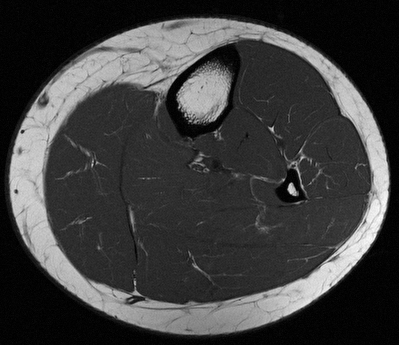
\includegraphics[width=.4\linewidth]{jambe.png}}
	\hfill
	\subfloat[Noisy image (salt and pepper).]{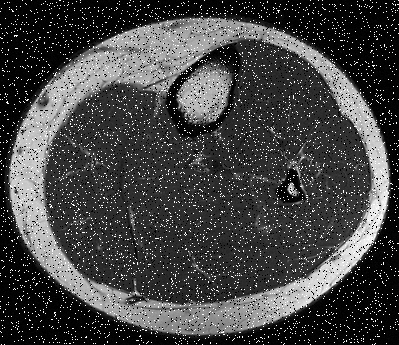
\includegraphics[width=.4\linewidth]{leg_sp.png}}
	
	\vspace*{-4pt}
	
	\subfloat[Maximum filter.]{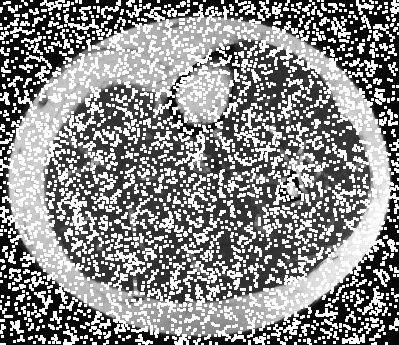
\includegraphics[width=.4\linewidth]{leg_maximum.png}}
	\hfill
	\subfloat[Minimum filter.]{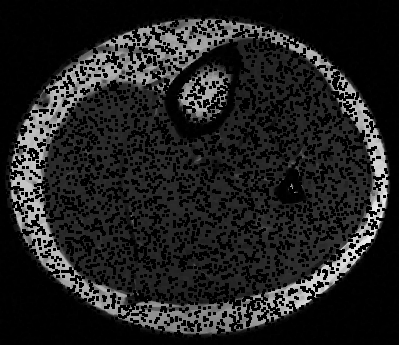
\includegraphics[width=.4\linewidth]{leg_minimum.png}}
	
	\vspace*{-4pt}
	
	\subfloat[Mean filter.]{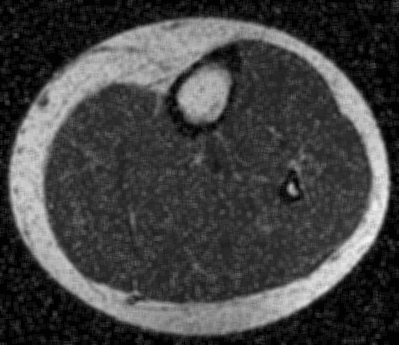
\includegraphics[width=.4\linewidth]{leg_uniform.png}}
	\hfill
	\subfloat[Median filter.]{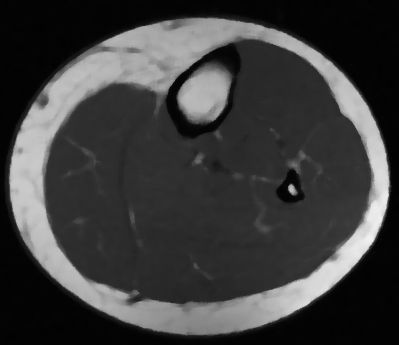
\includegraphics[width=.4\linewidth]{leg_median.png}}%
	\vspace*{-8pt}%
	\label{fig:image_restoration_denoising:python:filters}%
\end{figure}

\vspace*{-6pt}

\begin{python}
a = 0.05; b = 0.05;
spnoise = 0.5 * np.ones((nx,ny));
X = np.random.rand(nx,ny);
B = A.copy();
B[X<=a] = 0;
B[(X>a) & (X <= (a+b))] = 255;
fig = plt.figure()
plt.imshow(B, cmap='gray');
imageio.imwrite("leg_sp.png", B);
#plt.show()
\end{python}

Then, different filters are illustrated. Notice that the contours informations are somehow damaged. The median filter corresponds to the best filter in this case.

\begin{python}
### filtering by convolution
#average filtering
B1 = ndimage.uniform_filter(B,5);
imageio.imwrite("leg_uniform.png", B1);
B2 = ndimage.minimum_filter(B,3);
imageio.imwrite("leg_minimum.png", B2);
B3 = ndimage.maximum_filter(B,3);
imageio.imwrite("leg_maximum.png", B3);
B4 = ndimage.median_filter(B, 7);
imageio.imwrite("leg_median.png", B4);
B5 = amf(B, 7);
plt.imshow(B5, cmap='gray');
imageio.imwrite("leg_amf.png", B5);
\end{python}



What can be noticed is that min and max filters are unable to restore the image (opening and closing filters, from the mathematical morphology, could be a solution to explore). The mean filter is a better solution, but an average value is highly modified by an impulse noise. The median filter is the optimal solution is order to suppress the noise, but fine details are lost. An interesting solution is to apply an adaptive median filter. 

%\newpage
\subsubsection{Adaptive median filter}
The following code is a simple implementation of the algorithm previously presented. It has not been optimized in order to have a simple presentation. A more sophisticated version can be found in \cite{Gonzalez2002}. The results are illustrated in Fig.\ref{fig:image_restoration_denoising:python:amf_filter} for $S_{max}=7$.

\begin{python}
def amf(I, Smax):
    """
    Adaptive median filter
    I: grayscale image
    Smax: maximal size of neighborhood. Limits the effect of median filter
    """
    f = np.copy(I);
    nx, ny = I.shape;
    sizes = np.arange(1, Smax, 2);
    zmin = np.zeros((nx, ny, len(sizes)));
    zmax = np.zeros((nx, ny, len(sizes)));
    zmed = np.zeros((nx, ny, len(sizes)));
    for k,s in enumerate(sizes):
        zmin[:,:,k] = ndimage.minimum_filter(I, s);
        zmax[:,:,k] = ndimage.maximum_filter(I, s);
        zmed[:,:,k] = ndimage.median_filter (I, s);
    isMedImpulse = np.logical_or(zmin==zmed,zmax==zmed);
    
    for i in range(nx):
        for j in range(ny):
            k = 0;
            while k<len(sizes)-1 and isMedImpulse[i,j,k] :
                k+=1;
            
            if I[i,j] == zmin[i,j,k] or I[i,j]==zmax[i,j,k] or k==len(sizes):
                f[i,j] = zmed[i,j,k];
    return f;

\end{python}

\begin{figure}[ht]
 \centering\caption{Illustration of the adaptive median filter.}%
 \subfloat[Original image.]{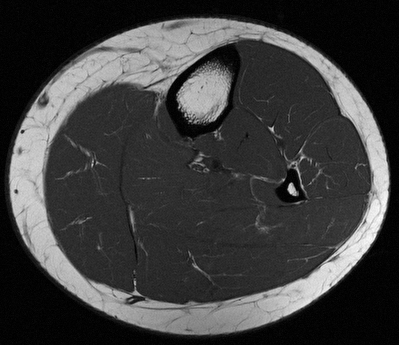
\includegraphics[width=.45\linewidth]{jambe.png}}
 \hfill
 \subfloat[Noisy image (salt and pepper).]{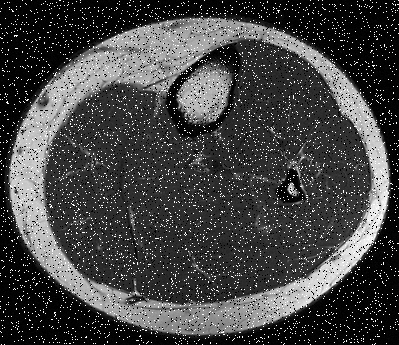
\includegraphics[width=.45\linewidth]{leg_sp.png}}
 
 \subfloat[Median filter of size $7\times 7$.]{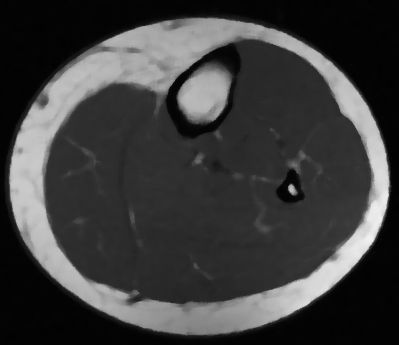
\includegraphics[width=.45\linewidth]{leg_median.png}}
 \hfill
 \subfloat[Adaptive median filter, $S_{max}=7$.]{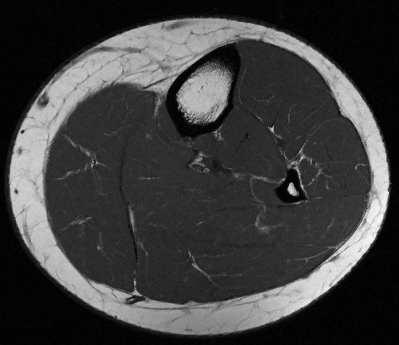
\includegraphics[width=.45\linewidth]{leg_amf.png}}%
 \label{fig:image_restoration_denoising:python:amf_filter}%
\end{figure}
